% IEEE standard conference template; to be used with:
%   spconf.sty  - LaTeX style file, and
%   IEEEbib.bst - IEEE bibliography style file.
% --------------------------------------------------------------------------

\documentclass[letterpaper]{article}
\usepackage{spconf,amsmath,amssymb,graphicx}
\usepackage{booktabs}
\usepackage{float}
\usepackage{xcolor}
\usepackage{listings}
\usepackage{pgf}

% Example definitions.
% --------------------
% nice symbols for real and complex numbers
\newcommand{\R}[0]{\mathbb{R}}
\newcommand{\C}[0]{\mathbb{C}}
\definecolor{listingbg}{RGB}{240, 240, 240}

% bold paragraph titles
\definecolor{intellijkeyword}{HTML}{000080}
\definecolor{intellijstrings}{HTML}{0000FF}
\definecolor{intellijcomment}{HTML}{008800}
\newcommand{\mypar}[1]{{\bf #1.}}
\lstset{ %
    backgroundcolor=,
    backgroundcolor=\color{listingbg},   	% choose the background color; you must add \usepackage{color} or \usepackage{xcolor}
    basicstyle=\footnotesize\ttfamily, 		% the size of the fonts that are used for the code
    breakatwhitespace=false,         		% sets if automatic breaks should only happen at whitespace
    breaklines=false,                 		% sets automatic line breaking
    captionpos=b,                    		% sets the caption-position to bottom
    commentstyle=\itshape\color{intellijcomment},   % comment style
    deletekeywords={...},            		% if you want to delete keywords from the given language
    escapeinside={\%*}{*)},          		% if you want to add LaTeX within your code
    extendedchars=true,              		% lets you use non-ASCII characters; for 8-bits encodings only, does not work with UTF-8
    frame=single,                    		% adds a frame around the code
    keepspaces=true,                 		% keeps spaces in text, useful for keeping indentation of code (possibly needs columns=flexible)
    keywordstyle=\bfseries\color{intellijkeyword},   % keyword style
    rulecolor=\color{listingbg},         	% if not set, the frame-color may be changed on line-breaks within not-black text (e.g. comments (green here))
    showspaces=false,                		% show spaces everywhere adding particular underscores; it overrides 'showstringspaces'
    showstringspaces=false,          		% underline spaces within strings only
    showtabs=false,                  		% show tabs within strings adding particular underscores
    stringstyle=\color{intellijstrings},    % string literal style
    title=\lstname,                   		% show the filename of files included with \lstinputlisting; also try caption instead of title
    belowskip=-2em,
}
\lstnewenvironment{ccode}{\lstset{language=C, numbers=left}}{}

%%% PATCH STARTS https://tex.stackexchange.com/questions/127667/matplotlib-pgf-images-in-subdirectory
\newcommand\inputpgf[2]{{
\let\pgfimageWithoutPath\pgfimage
\renewcommand{\pgfimage}[2][]{\pgfimageWithoutPath[##1]{#1/##2}}
\input{#1/#2}
}}

% Title.
% ------
\title{Bone Anisotropy Mapping}
%
% Single address.
% ---------------
\name{Jarunan Panyasantisuk, Joao Rivera, Rajan Gill, Ryan Cherifa } 
\address{Department of Computer Science\\ ETH Z\"urich\\Z\"urich, Switzerland}

% For example:
% ------------
%\address{School\\
%		 Department\\
%		 Address}
%
% Two addresses (uncomment and modify for two-address case).
% ----------------------------------------------------------
%\twoauthors
%  {A. Author-one, B. Author-two\sthanks{Thanks to XYZ agency for funding.}}
%		 {School A-B\\
%		 Department A-B\\
%		 Address A-B}
%  {C. Author-three, D. Author-four\sthanks{The fourth author performed the work
%		 while at ...}}
%		 {School C-D\\
%		 Department C-D\\
%		 Address C-D}
%

\begin{document}
%\ninept
%
\maketitle
%

\begin{abstract}
\color{red}{Todo}
\end{abstract}

\section{Introduction}\label{sec:intro}

Bone fabric anisotropy or microstructure orientation was recently included in finite element (FE) models to improve the accuracy in predicting bone stiffness and strength \cite{Maquer:2015, Musy:2017}. To save computing cost, an FE model of bone is generated from a clinical computer tomography (CT) scanned image with low resolution (1-3mm). However, the bone microstructure details can be obtained only by high resolution peripheral CT with the resolution of 60-82 $\mu$m. Therefore, bone anisotropy mapping methodology was required to map the bone microstructure orientation from the high resolution image onto the low resolution image.

Bone anisotropy mapping methodology includes coordinates mapping between a low and a high-resolution images, region extraction (RE), the mean intercept length (MIL) method for quantification of the microstructure orientation, ellipsoid fitting (EF) of MIL and eigendecomposition to obtain the major direction of the microstructure.

\mypar{Motivation} In the recent study, bone anisotropy mapping algorithms are performed for all low resolution image voxels and for all pairs (n=71) of low and high resolution images \cite{Panyasantisuk:18}. This preprocessing step consumes a significant amount of computing time. Moreover, researchers expect larger dataset to create a more general FE models of bone. Therefore, the performance of these algorithms are crucial. Two software packages for image processing which include MIL calculation are Medtool, a commercialized PYTHON package, and BoneJ, an open-source JAVA plugin for ImageJ. The external packages needed to be integrated to the computation pipeline and optimization is not straightforward. 

In this paper, we are presenting an integrated and optimized methodology of bone anisotropy mapping. At our best knowledge, this is the first paper to study and optimize the performance of MIL calculation depending on the extracted region size.
  
\section{Background}\label{sec:background}
% Coord mapping & region extraction
The methodology is shown in Fig.~\ref{fig:method}. Coordinates from a low resolution image were mapped to its own high resolution image. Then, a sphere region is extracted and centered at the mapped coordinate in the high resolution image. 
% MIL
Subsequently, the anisotropy of the extracted bone region is quantified by using MIL method which imposed direction vectors on the regions. The mean length of each vector is the sum of the length inside the bone region devided by the number of intercepts which intersect with bone/non-bone transition.
% ellipsoid fitting
The MIL values can be plots as a cloud of points in the direction vector space and an ellipsoid can be fitted to obtain a representative two dimensional tensor, for which three eigenvalues and three eigenvectors are calculated. The eigenvector associated with the minimum eigenvalue is the major direction of that bone region.

\begin{figure}[ht]
  \centering
  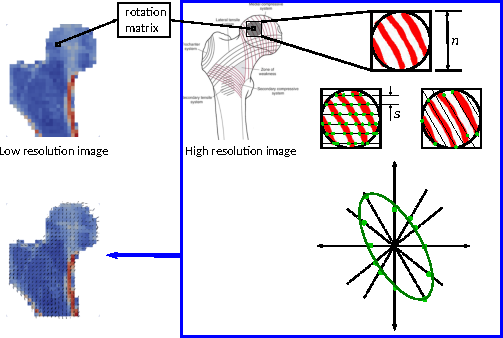
\includegraphics[width=3.25in]{figs/overview.pdf}
  \caption{Bone anisotropy mapping methodology includes coordinate mapping from low to high resolution image, RE from the high resolution image, MIL calculation, EF to obtain a fabric tensor and eigendecomposition of the fabric tensor from which the major eigenvector can be visualized. $n$ is the extracted region dimension in one direction. $s$ is the stride between parallel direction vectors.}
  \label{fig:method}
\end{figure}


\mypar{Region extraction (RE)}
This algorithm applies a sphere mask on the high resolution image and copies the extraction region to a separate array. A multiplication was performed for each image voxel.

\mypar{Mean Intercept Length (MIL) method}

% todo: add figure of MIL 
The mean intercept length of a vector ${v}$ can be expressed as
\begin{equation}
  MIL({v}) = \frac{h({v})}{C({v})},
\end{equation}
where $h(v)$ is the summation of the bone intensities ``touched" by all the rays formed by direction vector $v$, and $C(v)$ is the number of intercepts of the vector $v$.  In general, each ray is separated by a stride $s=2$. Thus, each direction vector touches only $\frac{n^3}{s^2}$ voxels in the region for $n$ even. We consider only $N_{vec}=13$ direction vectors.

As an example, consider the (2-D) extracted region in Fig~\ref{fig:method} with horizontal vector $\vec{v} = (1,0,0)$. In this region, $C({v})$ is the number of green dots, whereas $h({v})$ is calculated summing up all voxels touched by the horizontal doted lines.

%More precisely, let $R(\vec{v})$ be the set of rays formed by vector $\vec{v}$, where a ray $r\in R(\vec{v})$ is represented by the values of all voxels touched by such a ray. Thus, h and C can be calculated as follows:

The algorithm includes floating point additions to calculate $h({v})$ and comparisons to detect interceptions. Note that additions performed to calculate $C({v})$ are not considered in the cost analysis because those are performed over integers. In addition, one division is performed per direction vector. The total cost of the MIL algorithm per extracted region is therefore $C(n) = N_{vec}(\frac{2n^3}{s^2}+1)$. Table \ref{tab:cost} provides a detailed breakdown of the cost analysis.

% todo: algorithm for ellipsoid fitting
\mypar{Ellipsoid fitting (EF)}  
{\color{red}Todo}

%\begin{table}
%  \caption{Cost analysis}
%  \label{tab:cost}
%  \begin{tabular}{l c c c}
%    \toprule
%     & flops & read/write & Operational intensity\\
%     &   & [doubles] & [flops/double]\\
%    \midrule
%    Region extractions & $n^{3}$ & $3n^{3}$ & 1/3\\
%    MIL & $13(\frac{n^{3}}{2}+1)$ &  &  \\
%    Ellipsoid fitting\\
%    \bottomrule
%  \end{tabular}
%\end{table}

%{\color{red} Should we move this paragraph till the end (after we explain each algorithm)?}
From the basic implementation, MIL calculation, EF and RE consume approximately {\color{red} 80\%, 15\% and 5 \%} of the overall computing time, respectively. Therefore, we focused on these three algorithms for the optimization. The run time was measured by using time stamp counter (TSC).  We define our cost measure as the number of floating point operations (flops) performed by the algorithms. The cost analysis for each algorithm is shown in Table~\ref{tab:cost}, where $n$ is the size of the region extracted during RE. Note that each algorithm is performed once per non-zero voxel in the low resolution image. {\color{red} (This can be omitted)} Thus, the cost of the whole program is ${\color{red} total}\cdot N_{nz}$, where $N_{nz}$ is the number of non-zero voxels in the low resolution image which represent the bone voxel.

\begin{table}[H]
    \caption{Cost analysis per low-resolution bone voxel.}
    \label{tab:cost}
    \begin{tabular}{l c c c c | c}
        \toprule
        & $N_{add}$ & $N_{mul}$ & $N_{div}$ & $N_{cmp}$ & Total\\
        \midrule
        RE & - & $n^{3}$ & - & - &   $n^{3}$\\
        MIL & $\frac{13n^{3}}{4}$ & -  & 13 & $\frac{13n^{3}}{4}$ &  $13(\frac{n^{3}}{2}+1)$\\
        EF & & & & & \\
        \bottomrule
    \end{tabular}
\end{table}


\section{Methods}\label{sec:yourmethod}
%{\color{red} Add overview of the section}
% todo: 
% - basic implementation, quantify the perentage of each algorithm takes.
% - testing machine
This section explains the baseline implementation and optimization strategies of each focused algorithm.

\subsection{RE optimization} The baseline implementation loops over all voxels in the sphere mask with the size of $n^{3}$. For each sphere mask voxel, if a corresponding voxel in the high resolution image is found, the extracted region voxel is set as the multiplication of the sphere mask voxel and the high resolution image voxel. Therefore, loop unrolling with four parallel multiplications and scalar replacement were applied to speed up the computation and avoid aliasing. 

\subsection{MIL optimizations}
The following C-like pseudo code summarizes the baseline implementation of MIL algorithm:

\begin{ccode}[caption={My Caption},captionpos=b]
void mil_base(double* region, int n, double* mil){
  double h[13] = 0; int C[13] = 0;
  // Core of MIL
  for (int v = 0; v < 13; ++v)
    for every ray r of v  do
      {k,j,i} = get_start_of_ray(r);
      int prev = region[k][j][i];
      while ( {k,j,i} < n && {k,j,i} > 0 )
        h[v] += region[k][j][i];
        curr = region[k][j][i] > 0.5; // bone?
        C[v] += curr ^ prev; // interception
        prev = curr;
        {k,j,i} = next_voxel_indices({k,j,i}, v);
    mil[v] = h[v] / C[v];
 }
\end{ccode}
As can be seen, the baseline implementation iterates through all rays of all 13 direction vectors (see the \texttt{for} loop in lines 4-5). For each ray, we first get its starting voxel to begin iterating from (line 6). Finally, the inner loop iterates through the whole ray and computes $h(v)$ and $C(v)$. Note that $C(v)$ is an integer array; thus, the only floating point operations in this loop are the addition and comparison in lines 9-10.

\mypar{Improving ILP}
The first performance bottleneck in the baseline implementation is due to the non-associativity of floating point additions in line 9. This creates inter-loop dependencies between addition operations that limit the instruction level parallelism (ILP) of the implementation. Assuming a latency of floating point additions of 4 cycles, an upper bound on the performance due to this dependency is 0.5 flops/cycle (1 \texttt{add} + 1 \texttt{cmp} every 4 cycles).

In order to improve ILP, we used accumulators with loop-unrolling. We first unrolled the loop in line 5, to get four different rays of the same vector. We created an accumulator for each ray; thus, now we can perform 4 additions and 4 comparisons in parallel. Note that the rays for each accumulator should be of the same length to avoid handling leftovers at the end. For 1-Dimensional direction vectors, e.g. (1,0,0), all rays have the same length (equal to $n$); however, this is not the case for 2-D and 3-D vectors. Thus, we split the implementation for 1-D, 2-D and 3-D direction vectors in order to select a suitable set of rays of the same length for the inner most loop in each case.
{\color{red} If space, explain that the set of rays where chosen close to each other on the $x$ dimension to try to exploit some spacial locality.}

\mypar{Intensity analysis}
The second performance blocker are memory accesses. Assume that the extracted region is much larger than the size of the last level cache, i.e. $8n^3 >> N_{L3}$. For the first horizontal direction vector $v_1 = (1,0,0)$, a lower bound for the data read from memory is $Q_1(n) \geq \frac{n^3}{4}$ doubles. Recall that rays are spaced by a stride $s=2$; thus, not all data in the region is accessed by a vector. The bound of $Q_1(n)$ is close to tight for the horizontal vector because data is accessed sequentially for each ray. Thus, when a (mandatory) cache miss occurs, the data in the whole cache line that is brought to cache will be used in the following iterations taking advantage of spacial locality (except for the first or last cache line in the ray in case of misalignment). 

The second direction vector, $v_2 = (0,1,0)$, iterates through the extracted region vertically. Since we assumed a very large data-set, there is no reuse of data from the previous vector. Further, note that for the vertical vector, only half of the data in a cache line will be used in the best case due to the stride of $s=2$ for consecutive rays. Since unused data in a cache line still have to be read from memory, a lower bound for the data read for the vertical vector is $Q_2(n) \geq \frac{n^3}{2}$ doubles. The remaining vectors will behave similarly as the vertical vector. Hence, a lower bound for the total amount of data read from memory is $Q(n) \geq \frac{n^3}{4} + \frac{12n^3}{2} = 6.25n^3$. Recall from the cost analysis of the previous section that the total number of flops performed by MIL is $W(n)=13(\frac{n^{3}}{2}+1) \approx 6.5n^3$. An upper bound on the operation intensity of MIL for a large $n$ is therefore $I(n) \leq \frac{6.5n^3}{6.25n^3} = 1.04$ flops/double. We conclude that the implementation of the algorithm is memory bound when the data does not longer fit in the cache. 

\mypar{Blocking}
In order to improve the operational intensity and cache locality, the next optimization applied was blocking. The idea behind blocking is that we can improve on data reuse by partially calculating $h(v)$ and $C(v)$ in a cube-block of size $N_B^3$ that fits in L1 cache. Since the blocked data will still be in the cache for the next vector, data reuse will improve by taking advantage of spacial and temporal locality. Afterwards, we repeat this process for the next block until all the extracted region is covered. For simplicity, we assumed that the region size $n$ is divisible by the block size $N_B$.

There are two things to consider when implementing blocking for MIL. First, note that we are accessing the voxels in the extracted region that are touched by the rays of all direction vectors. To this end, the implementation first determines the start of a ray in the limits of the region to begin iterating from. When blocking, we have to pay special attention to choose the right starting points for the partial rays processed by each block. To illustrate this, consider Figure ??. The highlighted voxels are the starting points for each block. As can be seen, in this particular case, not all blocks have the same pattern for the starting points (see for example B1 and B2). This means that we would have to determine the start pattern for each block to implement blocking. Since we favor simplicity, we would like to have the same starting patter within all blocks. This is easy to achieve for 1-D and 2-D vectors by simply choosing $N_B$ multiple of the stride $s=2$. On the other hand, to achieve homogeneity between blocks when processing 3-D vectors, we had to change the starting pattern of the baseline implementation as shown in Figure ??.

The second aspect to consider when blocking is the correct initialization of \texttt{prev} variable (line 7 of listing ??) using the voxel before the start of the partial ray of the block. This is necessary to detect an interception at the start of the block. 

Assuming that the block fits completely in L1 cache, a lower bound for the data read from memory when processing a block is $Q_B(n) \geq N_B^3$ doubles. Ignoring conflict misses, this lower bound is tight. Since there are $\frac{n^3}{N_B^3}$ blocks in total, the amount of data read from memory to process the whole region using blocking is bounded by $Q(n) \geq N_B^3 \cdot \frac{n^3}{N_B^3} = n^3$ doubles. An upper bound on the operational intensity is therefore $I(n) \leq \frac{6.5n^3}{n^3} = 6.5$ flops/double. Thus, the implementation now became \textit{compute bound}. For the final implementation, we choose $N_B = 16$ which is the size that achieves the best performance.

\mypar{SIMD vectorization}
After using blocking to improve locality, we vectorized the code using SIMD instructions. Recall that four accumulators were used to improve ILP in the first optimization. Since the data is in double precision, we can store the accumulators in a SIMD AVX register and apply vector instructions. We also used loop unrolling to expose an additional rays that can be handled in a vector, therefore improving ILP. Note that we always choose rays with the same length to avoid the overhead of handling leftovers. Similar to the scalar version, the implementation for 1-D, 2-D and 3-D direction vectors are treated separately to choose suitable rays for each case. In summary, in most cases we are procession 8 rays simultaneously per loop iteration, stored in two SIMD register. The only exception is 3-D vectors in which processing 12 rays simultaneously in three SIMD registers was a more suitable option. 
Figure \ref{fig:simd_mil} shows the vectorized diagram for the main operations used in MIL.
It is also worth noting that 3-D direction vectors have inherently more overhead that 2-D or 1-D vectors because they have more and shorter rays. Thus, there is more overhead when determining the starting points for the next set of rays to be processed.

\begin{figure}[H]
    \centering
    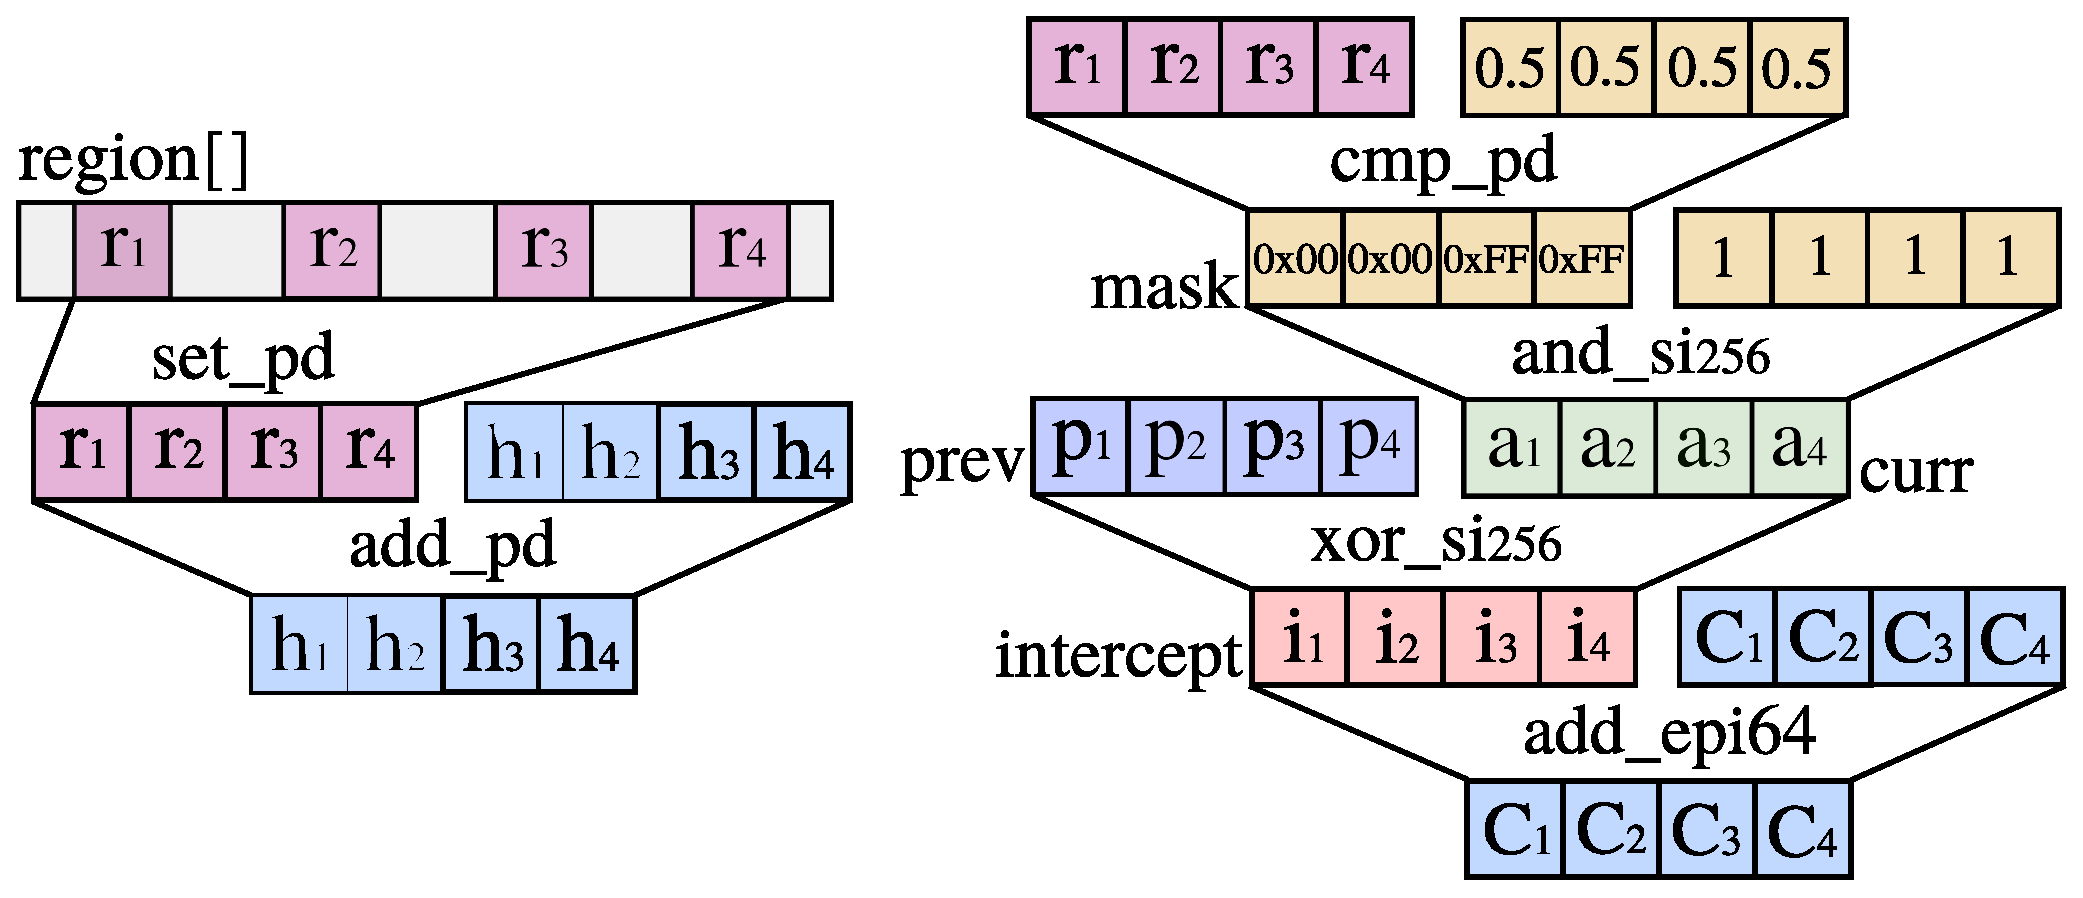
\includegraphics[width=3.4in]{figs/simd_mil2.eps}
    \caption{SIMD vectorization of four rays in MIL.}
    \label{fig:simd_mil}
\end{figure}


\subsection{EF} moving loop invariant code, SIMD


\section{Experimental Results}\label{sec:exp}

The experimental results are presenting here according to the algorithms.

\mypar{RE} \textit{Experimental setup} The tests were performed on Intel i7 U7600 (Kaby Lake), 2.8 GHz without Turboboost. The L1, L2 and L3 cache size were 32KB, 256KB, and 8MB, respectively. The highest optimization flag was used without vectorization (\texttt{-O3 -fno-vectorize-tree}). The sphere region size were ranged from $n=8^{3}$ to $128^{3}$.

\textit{Results} As seen in Fig.~\ref{res:regions}, the loop unrolling and scalar replacement did not improve the performance for the region extraction algorithms. The compiler might already perform well in alias checking and parallelizing the multiplications. When the extracted region size fitted in the cache, the performance was bound to 1 flops/cylce due to the instruction combinations. On the other hand, when the extracted region size was too large for the cache, the performance was bound to 0.5 flops/cycle due to the memory. The results shows that the algoirthm reached around 0.8 flops/cycle in the cache and stayed around 0.2 flops/cycle in the memory.
   
\begin{figure}[H]
  \centering
 
  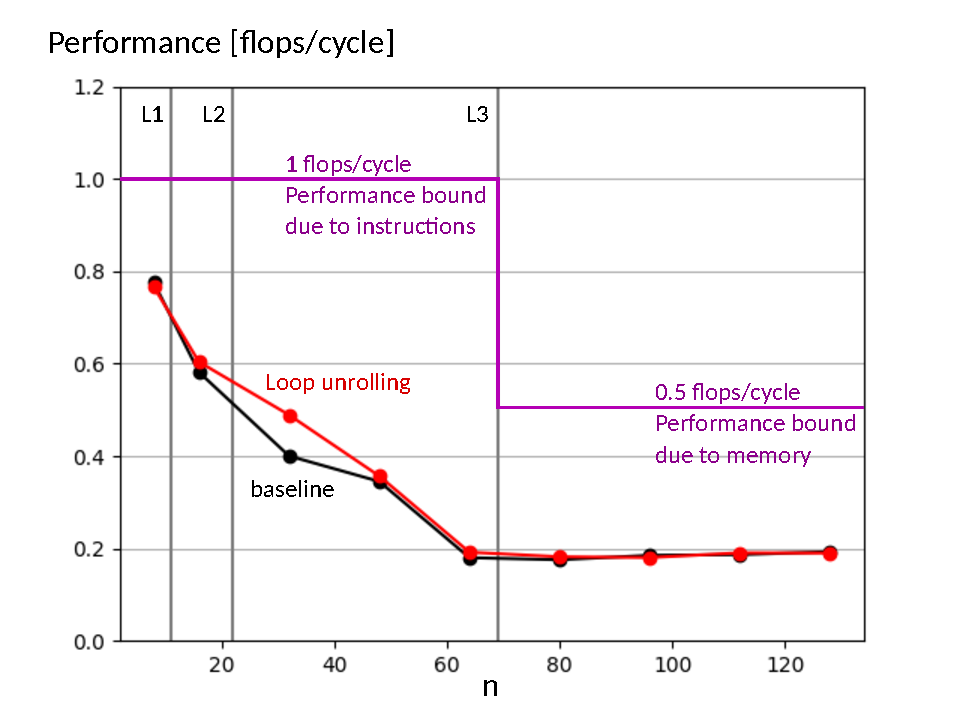
\includegraphics[width=3.5in]{figs/plots/regions/regions_performance.pdf}
  \caption{Performance of RE}
  \label{res:regions}
\end{figure}


\mypar{MIL} \textit{Experimental setup}

\textit{Results}

\begin{figure}[H]
  \centering
  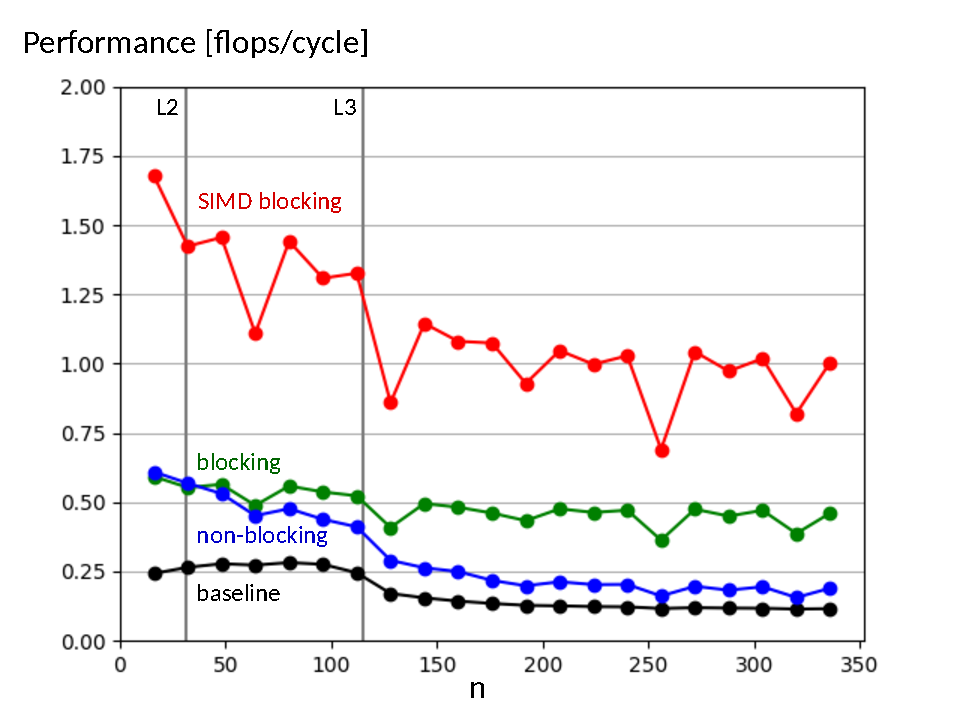
\includegraphics[width=3.5in]{figs/plots/mil/mil_performance.pdf}
  \caption{Performance of MIL}
  \label{res:mil}
\end{figure}

\textit{Conflict Misses}

\begin{figure}[H]
  \inputpgf{figs/conflict_miss}{mil_blocking_conflicts_64.pgf}\vspace{-1cm}
  \caption{Cache line mappings for the first 16x16x16 block of a 64x64x64 region (all units are in doubles). Note that a single cache block is 8 doubles. The grey circle represents the start of a cache block. The numbers represent the cache line numbers for the associated $i,j$ entry and for $k=0,1,2,3,...$. }
  \label{res:conflict_miss_64}
\end{figure}
\begin{figure}[H]
  \inputpgf{figs/conflict_miss}{mil_blocking_conflicts_65.pgf}\vspace{-1cm}
  \caption{Cache line mappings for the first 16x16x16 block of a 65x65x65 region (all units are in doubles). Note that a single cache block is 8 doubles. The grey circle represents the start of a cache block. The numbers represent the cache line numbers for the associated $i,j$ entry and for $k=0,1,2,3,...$. }
  \label{res:conflict_miss_65}
\end{figure}

\mypar{EF} \textit{Experimental setup}

\textit{Results}
 
\begin{figure}[H]
  \centering 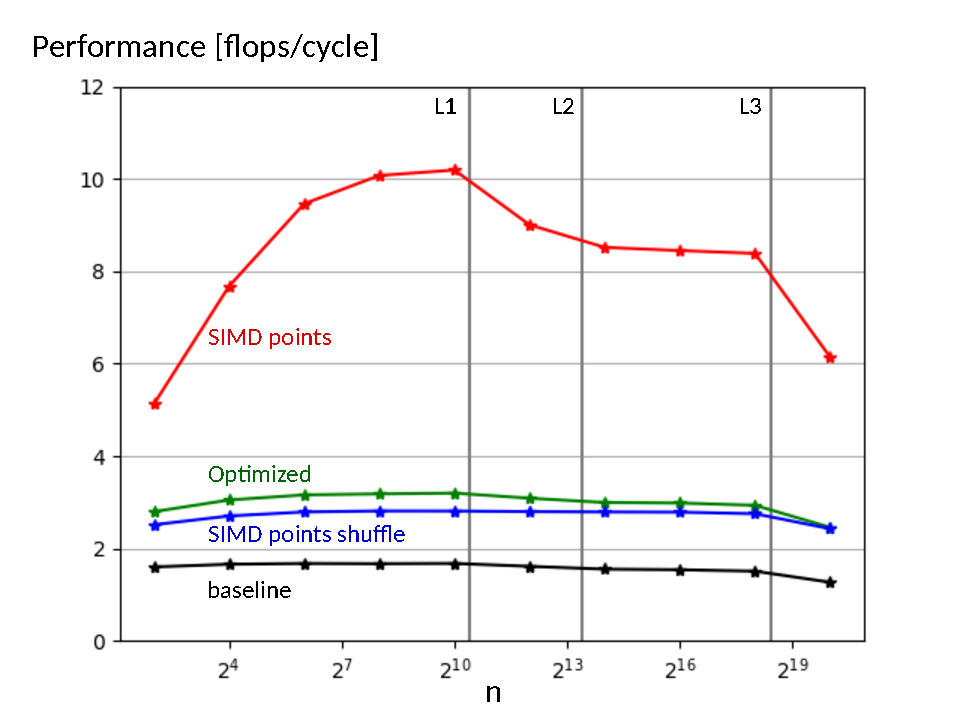
\includegraphics[width=3.5in]{figs/plots/ellipsoid/ellipsoid_performance.pdf}
  \caption{Performance of EF}
  \label{res:ellipsoid}
\end{figure}


\mypar{Overall performance}

\section{Conclusions}

The bone anisotropy mapping was integrated and optimized. MIL calculation consumes the large percentage of the overall computation time, followed by EF and RE. 

The performance of RE was bounded by the intructions mix when it was in cache and memory bound when in memory. The loop unrolling did not improve the performance and the compiler already optimized the alias checking in the basic implementation.

MIL calculation\\

EF\\


\section{Further comments}

Here we provide some further tips. 

\mypar{Further general guidelines}

% References should be produced using the bibtex program from suitable
% BiBTeX files (here: bibl_conf). The IEEEbib.bst bibliography
% style file from IEEE produces unsorted bibliography list.
% -------------------------------------------------------------------------
\bibliographystyle{IEEEbib}
\bibliography{bibl_conf}

\end{document}

